\documentclass{article}

\usepackage{fancyhdr}
\usepackage{extramarks}
\usepackage{amsmath}
\usepackage{amsthm}
\usepackage{amsfonts}
\usepackage{tikz}
\usepackage[plain]{algorithm}
\usepackage{algpseudocode}

\usetikzlibrary{automata,positioning}

%
% Basic Document Settings
%

\topmargin=-0.45in
\evensidemargin=0in
\oddsidemargin=0in
\textwidth=6.5in
\textheight=9.0in
\headsep=0.25in

\linespread{1.1}

\pagestyle{fancy}
\lhead{\hmwkAuthorName}
\chead{\hmwkClass\ (\hmwkClassInstructor\ \hmwkClassTime): \hmwkTitle}
\rhead{\firstxmark}
\lfoot{\lastxmark}
\cfoot{\thepage}

\renewcommand\headrulewidth{0.4pt}
\renewcommand\footrulewidth{0.4pt}

\setlength\parindent{0pt}

%
% Create Problem Sections
%

\newcommand{\enterProblemHeader}[1]{
    \nobreak\extramarks{}{Problem \arabic{#1} continued on next page\ldots}\nobreak{}
    \nobreak\extramarks{Problem \arabic{#1} (continued)}{Problem \arabic{#1} continued on next page\ldots}\nobreak{}
}

\newcommand{\exitProblemHeader}[1]{
    \nobreak\extramarks{Problem \arabic{#1} (continued)}{Problem \arabic{#1} continued on next page\ldots}\nobreak{}
    \stepcounter{#1}
    \nobreak\extramarks{Problem \arabic{#1}}{}\nobreak{}
}

\setcounter{secnumdepth}{0}
\newcounter{partCounter}
\newcounter{homeworkProblemCounter}
\setcounter{homeworkProblemCounter}{1}
\nobreak\extramarks{Problem \arabic{homeworkProblemCounter}}{}\nobreak{}

%
% Homework Problem Environment
%
% This environment takes an optional argument. When given, it will adjust the
% problem counter. This is useful for when the problems given for your
% assignment aren't sequential. See the last 3 problems of this template for an
% example.
%
\newenvironment{homeworkProblem}[1][-1]{
    \ifnum#1>0
        \setcounter{homeworkProblemCounter}{#1}
    \fi
    \section{Problem \arabic{homeworkProblemCounter}}
    \setcounter{partCounter}{1}
    \enterProblemHeader{homeworkProblemCounter}
}{
    \exitProblemHeader{homeworkProblemCounter}
}

%
% Homework Details
%   - Title
%   - Due date
%   - Class
%   - Section/Time
%   - Instructor
%   - Author
%

\newcommand{\hmwkTitle}{Homework 3}
\newcommand{\hmwkDueDate}{Feburary 12, 2020}
\newcommand{\hmwkClass}{Physics 216}
\newcommand{\hmwkClassTime}{Section 509}
\newcommand{\hmwkClassInstructor}{Dr. Ostrovskaya}
\newcommand{\hmwkAuthorName}{\textbf{Amari West}}
\newcommand{\hmwkDueTime}{11:59pm}

%
% Title Page
%

\title{
    \vspace{2in}
    \textmd{\textbf{\hmwkClass:\ \hmwkTitle}}\\
    \normalsize\vspace{0.1in}\small{Due\ on\ \hmwkDueDate\ at \hmwkDueTime}\\
    \vspace{0.1in}\large{\textit{\hmwkClassInstructor\ \hmwkClassTime}}\\
    \vspace{3in}\textbf{Pages: 13}
}

\author{\hmwkAuthorName}
\date{}

\renewcommand{\part}[1]{\textbf{\large Part \Alph{partCounter}}\stepcounter{partCounter}\\}

%
% Various Helper Commands
%

% Useful for algorithms
\newcommand{\alg}[1]{\textsc{\bfseries \footnotesize #1}}

% For derivatives
\newcommand{\deriv}[1]{\frac{\mathrm{d}}{\mathrm{d}x} (#1)}

% For partial derivatives
\newcommand{\pderiv}[2]{\frac{\partial}{\partial #1} (#2)}

% Integral dx
\newcommand{\dx}{\mathrm{d}x}

% Alias for the Solution section header
\newcommand{\solution}{\textbf{\large Solution}}

% Probability commands: Expectation, Variance, Covariance, Bias
\newcommand{\E}{\mathrm{E}}
\newcommand{\Var}{\mathrm{Var}}
\newcommand{\Cov}{\mathrm{Cov}}
\newcommand{\Bias}{\mathrm{Bias}}

% Allow double underline
\def\doubleunderline#1{\underline{\underline{#1}}}

% Allow for units in math mode
\newcommand{\unit}[1]{\ensuremath{\, \mathrm{#1}}}

\begin{document}

\maketitle

\pagebreak

\begin{homeworkProblem}
	A certain type of storage battery lasts on the average 3.0 years, with a standard deviation of 0.5 year. Assuming that the battery lives are normally distributed, find the probability that a given battery will last less than 2.3 years.
	\\
	\\
	
	\textbf{\underline{Given}}
	\begin{itemize}
		\item $\mu = 3.0 \unit{years}$
		\item $\sigma = 0.5 \unit{years}$
		\item $x = 2.3 \unit{years}$
	\end{itemize}

	\textbf{\underline{Find}}
	\\
	
	The probability that a given battery will last less than 2.3 years. 
	\\
	\\
	
	\textbf{\underline{Diagram}}
	
	\includegraphics[scale=0.9]{problem1}
	
	\textbf{\underline{Theory}}
	\\
	
	To find the probability of a battery will die within the specified range of duration, a $z$-value must be found with the following formula and used with a $z$-table.
	
	\[
	z = \frac{x - \mu}{\sigma}
	\]
	
	Since the range in question does not contain the average, $P(2.3 < x < 3.0)$ will be subtracted from $P(0.0 < x < 3.0)$ which has a $z$-value equal to 0.5. Once this has been done, the probability can be calculated.
	\\
	\\
	
	\textbf{\underline{Assumptions}}
	\\
	
	The normal lifespan of a battery is $N(3.0,(0.5)^{2})$.
	\\
	\\
	
	\textbf{\underline{Solution}}
	\\
	
	First, calculate $z$
	
	\[
	\begin{split}
		z &= \frac{2.3 - 3.0}{0.5}
		\\
		&= 1.4
	\end{split}
	\]
	
	Find the $z$-value
	
	\[
	\begin{split}
		P(0.0 < x < 2.3) &= 0.5 - P(0.0 < z < 1.4)
		\\
		&= 0.5 - 0.4192
		\\
		&= \doubleunderline{0.0808}
	\end{split}
	\]
	
	\textbf{\underline{Conclusion}}
	\\
	
	The probability that a battery will last between 0.0 hours and 2.3 years is \boxed{8.1\%.}
	
\end{homeworkProblem}

\pagebreak

\begin{homeworkProblem}
	An electrical firm manufactures light bulbs that have a length of life that is normally distributed with mean equal to 800 hours and a standard deviation of 40 hours. Find the probability that a bulb burns between 778 and 834 hours.
	\\
	\\
	
	\textbf{\underline{Given}}
	\begin{itemize}
		\item $\mu = 800 \unit{hours}$
		\item $\sigma = 40 \unit{hours}$
		\item $x_{1} = 778 \unit{hours}$
		\item $x_{2} = 834 \unit{hours}$
	\end{itemize}
	
	\textbf{\underline{Find}}
	\\
	
	The probability of a bulb that burns between 778 hours and 834 hours within a population using a z-table that does not include the left half of the area under a bell curve. \\
	
	\textbf{\underline{Diagram}}
	
	\includegraphics[scale=0.90]{problem2}
	
	\textbf{\underline{Theory}}
	\\
	
	To find the probability of a bulb will burn within the specified range of duration, a $z$-value must be found with the following formula and used with a $z$-table.
	
	\[
		z = \frac{x - \mu}{\sigma}
	\]
	
	
	However, since the z-table used only deals with half of the curve, two separate z calculations must be made, using
	
	\[
		z_{1} = \frac{x_{1} - \mu}{\sigma}	
	\]
	
	and 
	
	\[
		z_{2} = \frac{x_{2} - \mu}{\sigma}
	\]
	
	Once the $z$-values have been calculated, they can be added together to find the probability or $\int_{z_{1}}^{z_{2}} f(z) dz$ of the curve. 
	\\
	\\
	
	\textbf{\underline{Assumptions}}
	\\
	
	The normal burn time for these light bulbs is $N(800,(40)^{2})$
	\\
	\\
	
	\textbf{\underline{Solution}}
	\\
	
	First, calculate $z_{1}$
	
	\[
	\begin{split}
		z_{1} &= \frac{834 - 800}{40}
		\\
		&= 0.85
	\end{split}
	\]
	
	Next, calculate $z_{2}$
	
	\[
	\begin{split}
		z_{2} &= \frac{778 - 800}{40}
		\\
		&= 0.55
	\end{split}
	\]
	
	Use the $z$-table to find the area under the curve for both values. Note: since the $z$-table only deals with half of the curve each side is calculated separately.
	
	\[
	\begin{split}
		P(778 < x < 800) &= P(0.55 < z < 0.85)
		\\
		&= P(0.55 < z) + P(0.85 > z)
		\\
		&= .2088 + .3023
		\\
		&= \doubleunderline{0.5111}
	\end{split}
	\]
	
	\textbf{\underline{Conclusion}}
	\\
	
	The probability that a light bulb will burn between 778 hours and 800 hours is \boxed{51.1\%.}
	
	
\end{homeworkProblem}

\pagebreak

\begin{homeworkProblem}
	In an industrial process the diameter of a ball bearing is an important component part. They buyer sets specifications on the diameter to be $3.0 \pm 0.01$ cm. The implication is that no part falling outside these specifications will be accepted. It is known that in the process the diameter of a ball bearing has a normal distribution with mean 3.0 and standard deviation $\sigma = 0.005$. On the average, how many manufactured ball bearings will be scrapped?
	\\
	\\
	
	\textbf{\underline{Given}}
	\begin{itemize}
		\item $\mu = 3.0 \unit{cm}$
		\item $\sigma = 0.005 \unit{cm}$
		\item $x_{1} = 2.99 \unit{cm}$
		\item $x_{2} = 3.01 \unit{cm}$
		\item Acceptable Value = $3.0 \pm 0.01 \unit{cm}$ 
 	\end{itemize}
 
 	\textbf{\underline{Find}}
 	\\
 	\\
 	The probability that the manufactured ball bearings will be scrapped.
 	\\
 	\\
 	
 	\textbf{\underline{Diagram}}
 	
 	\includegraphics[scale=0.90]{problem3}
 
 	\pagebreak
 	
 	\textbf{\underline{Theory}}
 	\\
 	
 	To find the probability of creating a ball bearing with a diameter outside of specified range, a $z$-value must be found with the following formula and used with a $z$-table.
 	
 	\[
 	z = \frac{x - \mu}{\sigma}
 	\]
 	
 	Since both ranges are at the same distance from the mean, it is possible to find a single probability using only one of the $x$-values and multiply that probability by 2 to get the final answer. This is possible due to the fact that the $z$-table in use only handles half of the curve.
 	\\
 	\\
 	
 	\textbf{\underline{Assumptions}}
 	\\
 	
 	The normal diameter of these ball bearings is $N(3.0,(0.005)^{2})$
 	\\
 	\\
 	
 	\textbf{\underline{Solution}}
 	\\
 	
 	First, find the respective $z$-values using $x_{1}$ and $x_{2}$
 	
 	\[
 	\begin{split}
	 	z &= \frac{3.01 - 3.0}{0.005}
	 	\\
	 	&= 2
 	\end{split}
 	\]
 	
 	\[
 	\begin{split}
 	z &= \frac{2.99 - 3.0}{0.005}
 	\\
 	&= -2
 	\end{split}
 	\] 
 	
 	Next, find the probability and subtract it from 0.5, but due to symmetry this is done twice. The negative 2 is turned into a positive since there are no negatives on the $z$-table that is used.
 	
 	\[
 	\begin{split}
 		P(x < 2.99 \cup 3.01 < x) &= 2(0.5) - P(2 < z)
 		\\
 		&= 2(0.5 - .4772)
 		\\
 		&= 1 - 0.9544
 		\\
 		&= \doubleunderline{0.0456}
 	\end{split}
 	\]
 	
	\textbf{\underline{Conclusion}}
	\\
	
	According to the calculations, \boxed{4.56\%} of the ball bearings will be removed.
 	
\end{homeworkProblem}

\pagebreak

\begin{homeworkProblem}
	Gauges are used to reject all components in which a certain dimension is not within the specification $1.50 \pm d$. It is known that this measurement is normally distributed with mean 1.50 and standard deviation 2.0. Determine the value $d$ such that the specifications "cover" 95\% of the measurements.
	\\
	\\
	
	\textbf{\underline{Given}}
	\\
	\begin{itemize}
		\item $\mu = 1.50$
		\item $\sigma = 2.0$
		\item $x_{1} = 1.50 - d$
		\item $x_{2} = 1.50 + d$
		\item Probability = 95\%
	\end{itemize}

	\textbf{\underline{Find}}
	\\
	\\
	The value of $d$ such that specifications include 95\% of the measurements.
	\\
	\\
	
	\textbf{\underline{Diagram}}
	
	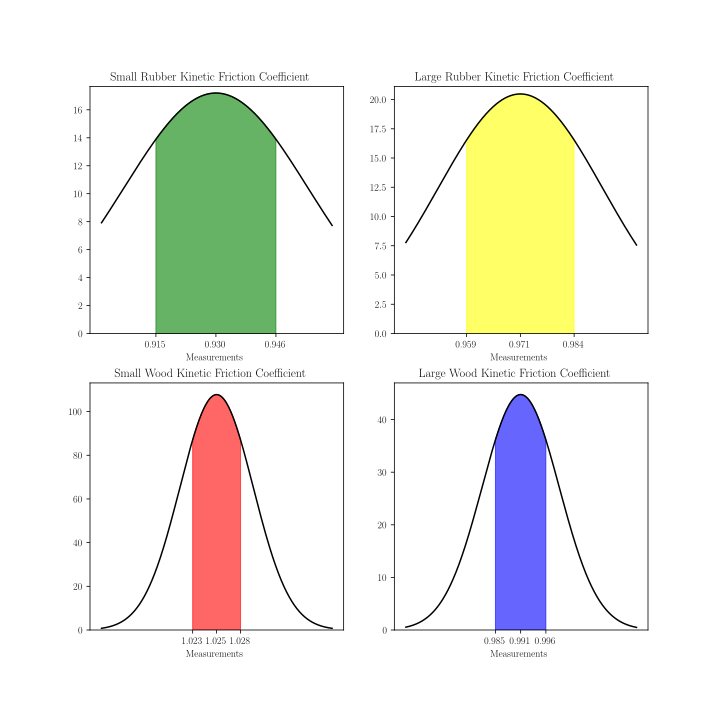
\includegraphics[scale=.90]{problem4}
	
	\textbf{\underline{Theory}}
	\\
	
	To find the value of $d$, the following formula may be used.
	
	\[
	z = \frac{x - \mu}{\sigma}
	\]
	
	Since the probability is already given, the $z$-table can be used backwards to find the appropriate $z$-value, and the formula above can be reconfigured to find $d$.
	\\
	\\
	
	\textbf{\underline{Assumptions}}
	\\
	\\
	The normal value of the measurements is $N(1.50,(2.0)^{2})$
	\\
	\\
	
	\textbf{\underline{Solution}}
	\\
	
	First, plug in $x_{2}$ into the equation used to find $z$ and use \underline{half} of the given percentage, 95\%, to find the $z$-value to plug in as $z$.
	
	\[
	\begin{split}
		1.96 &= \frac{(1.50 + d) - 1.50}{2.0}
		\\
		&= \frac{d}{2.0}
	\end{split}
	\]
	
	Now, solve for $d$
	
	\[
	\begin{split}
		d &= (1.96)(2.0)
		\\
		&= \doubleunderline{0.392}
	\end{split}
	\]   	
	
	\textbf{\underline{Conclusion}}
	\\
	\\
	The value for $d$ is \boxed{0.392.}
\end{homeworkProblem}

\pagebreak

\begin{homeworkProblem}
	A certain machine makes electrical resistors having a mean resistance of 40 ohms and a standard deviation of 2 ohms. Assuming that the resistance follows a normal distribution and can be measured to any degree of accuracy, what percentage of resistors will have a resistance that exceeds 43 ohms?
	\\
	\\
	
	\textbf{\underline{Given}}
	\begin{itemize}
		\item $\mu = 40 \unit{\Omega}$
		\item $\sigma = 2 \unit{\Omega}$
		\item $x = 43 \unit{\Omega}$
	\end{itemize}
	
	\textbf{\underline{Find}}
	\\
	
	The percentage of resistors that will have a resistance over 43 $\Omega$.
	\\
	\\
	
	\textbf{\underline{Diagram}}
	
	\includegraphics[scale=.9]{problem5}
	
	\textbf{\underline{Theory}}
	\\
	
	To find the probability of a resistor with a resistance over 45 $\Omega$, a $z$-value must be found with the following formula and used with a $z$-table.
	
	\[
	z = \frac{x - \mu}{\sigma}
	\]
	
	Since the range in question does not contain the average, $P(43 < x < \infty)$ will be subtracted from $P(40 < x < \infty)$ which has a $z$-value equal to 0.5. Once this has been done, the probability can be calculated.
	\\
	\\
	
	\textbf{\underline{Assumptions}}
	\\
	
	The normal value of resistance is $N(40,(2)^{2})$
	\\
	\\
	
	\textbf{\underline{Solution}}
	\\
	
	First, calculate $z$
	
	\[
	\begin{split}
		z &= \frac{43 - 40}{2}
		\\
		&= 1.5
	\end{split}
	\]
	
	Find the $z$-value
	
	\[
	\begin{split}
		P(43 < x < \infty) &= 0.5 - P(0.0 < z < 1.5)
		\\	
		&= 0.5 - 0.4332
		\\
		&= \doubleunderline{0.0668}
	\end{split}
	\]
	
	\textbf{\underline{Conlcusion}}
	\\
	
	The probability of the resistance being over 43 $\Omega$ is \boxed{6.68\%.}
	
\end{homeworkProblem}

\pagebreak

\begin{homeworkProblem}
	On an examination the average grade was 74 and the standard deviation was 7. If 12\% of the class are given A's, and the grades are curved to follow a normal distribution, what's the lowest possible A and the highest possible B? What is the sixth decile?
	\\
	\\
	
	\textbf{\underline{Given}}
	\begin{itemize}
		\item $\mu = 74$
		\item $\sigma = 7$
		\item 12\% of students made an A
	\end{itemize}

	\textbf{\underline{Find}}
	\begin{itemize}
		\item The value of $x$
		\item Lowest possible A
		\item Highest possible B
		\item The probability that a person scored within the sixth decile
	\end{itemize}

	\textbf{\underline{Diagram}}
	
	\includegraphics[scale=.9]{problem6}
	
	\textbf{\underline{Theory}}
	\\
	
	To find the value of the lowest A and highest B, the following formula may be used to $x$ which would lead to the answers. Since area of 0.12 is already given, it can be subtracted from 0.5 to get a new value that should then assist in finding the $z$-value
	
	\[
	x = \sigma z + \mu
	\]
	
	To find the sixth decile, the value of 0.1 can be used to find a desired $z$-value which could then be plugged into the formula above.
	\\
	\\
	
	\textbf{\underline{Assumptions}}
	\\
	
	The normal value of resistance is $N(74,(7)^{2})$
	\\
	\\
	
	\textbf{\underline{Solution}}
	\\
	
	\textbf{Part A}
	
	To find the lowest A and highest B, first subtract 0.12 from 0.50
	
	\[
		0.50 - 0.12 = 0.38
	\]
	
	Plug in the new value into the $z$-table to get 1.18, and use this value to find $x$
	
	\[
	\begin{split}
		x &= (7)(1.18) + 74
		\\
		&= \doubleunderline{82.26}
	\end{split}
	\]
	
	This $x$ value shows that the lowest A is 83 and the highest B is 82
	
	\textbf{Part B}
	
	To find the grade that marks the sixth decile, first use the $z$-table to plug in 0.10 to find 0.26. Now plug it into the above equation to find the solution.
	
	\[
	\begin{split}
		x &= (7)(0.26) + 74
		\\
		&= \doubleunderline{75.82}
	\end{split}
	\]
	
	Therefore $D_{6} = 75.82$.
	\\
	\\
	
	\textbf{\underline{Conclusion}}
	\\
	
	The lowest A is \boxed{83} and the highest B is \boxed{82} and the sixth decile is \boxed{75.82.}
	
\end{homeworkProblem}
\end{document}
